\documentclass{article}
\usepackage{tikz}

\begin{document}

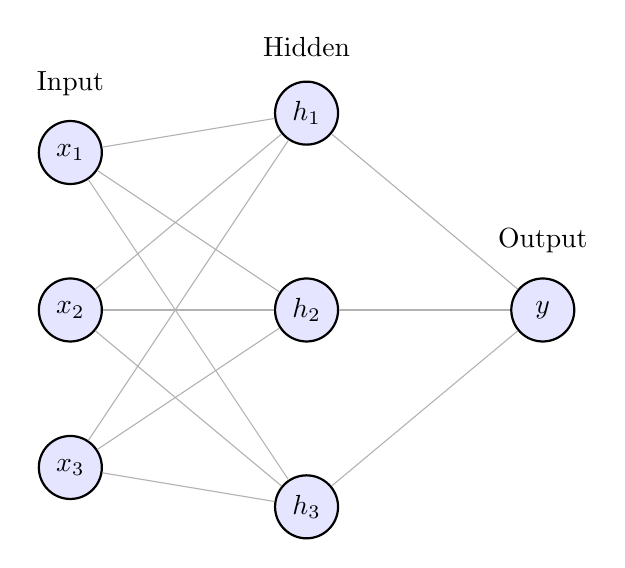
\begin{tikzpicture}[
    neuron/.style={
        circle,
        draw,
        thick,
        minimum size=8mm,
        fill=blue!10
    }
]

% Input layer
\node[neuron] (I1) at (0,2) {$x_1$};
\node[neuron] (I2) at (0,0) {$x_2$};
\node[neuron] (I3) at (0,-2) {$x_3$};

% Hidden layer
\node[neuron] (H1) at (3,2.5) {$h_1$};
\node[neuron] (H2) at (3,0) {$h_2$};
\node[neuron] (H3) at (3,-2.5) {$h_3$};

% Output
\node[neuron] (O) at (6,0) {$y$};

% Input → hidden
\foreach \i in {1,2,3}
    \foreach \h in {1,2,3}
        \draw[gray!60] (I\i) -- (H\h);

% Hidden → output
\foreach \h in {1,2,3}
    \draw[gray!60] (H\h) -- (O);

% Layer labels
\node[above] at (0,2.6) {Input};
\node[above] at (3,3.1) {Hidden};
\node[above] at (6,0.6) {Output};

\end{tikzpicture}

\end{document}
